\chapter{Ambiente de Engenharia AOSP Android 15 e Política de Documentação}
\label{chap:aosp_android15}

\begin{pedagogico}{Objetivo e Relevância no Android 15}
Este capítulo documenta a infraestrutura de compilação, desenvolvimento de daemons nativos e execução emulada para o \textbf{Android 15 (Vanilla Ice Cream / API 35)}. Aborda a transição mandatória para o \textbf{AIDL NDK Backend}, o isolamento por \textbf{SELinux Treble} e estabelece o rigoroso \textbf{Quality Gate de Documentação Obrigatória de Features} implementado neste repositório.
\end{pedagogico}

\section{Fundamentação da Árvore AOSP Android 15}

Com a chegada do Android 15, a Google consolidou o modelo de desenvolvimento contínuo \textit{Trunk-Stable}. Diferente das versões legadas onde o código era fragmentado por ramificações semestrais, no Android 15 as novas capacidades de sistema são ativadas seletivamente por \textit{build flags} no target de compilação (\texttt{trunk\_staging}).

\begin{figure}[htbp]
    \centering
    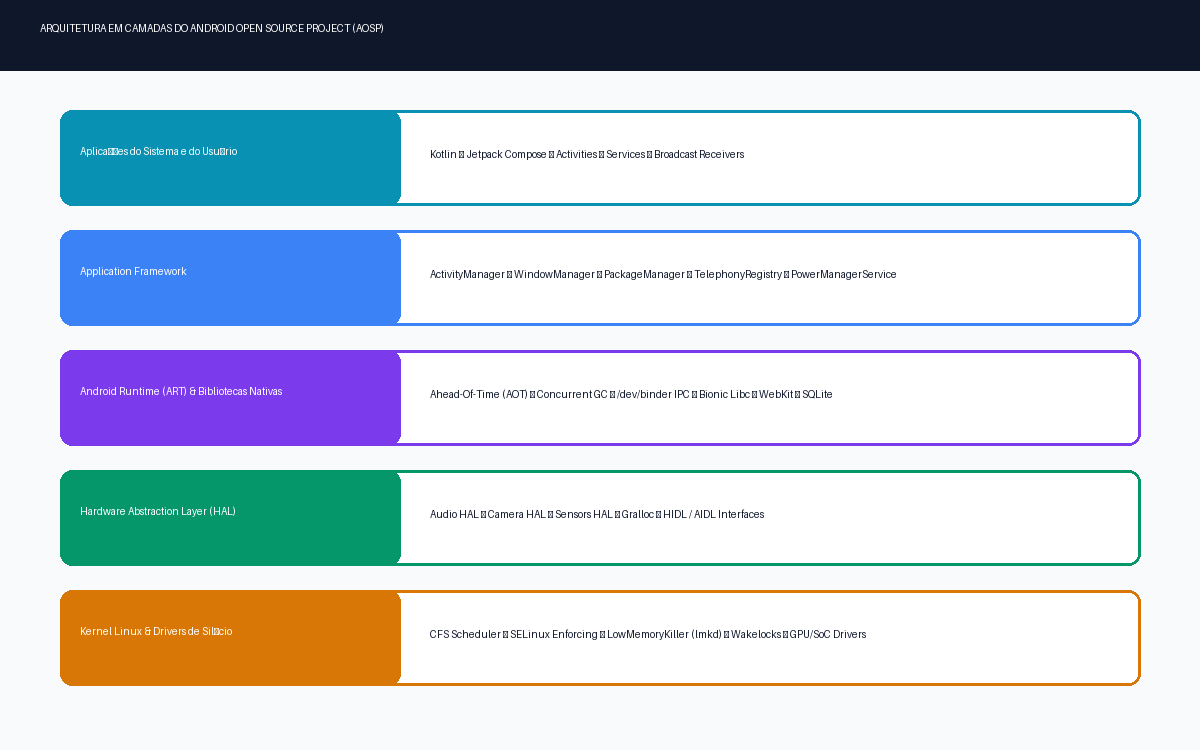
\includegraphics[width=0.85\textwidth]{imagens/fig_aosp_arquitetura.png}
    \caption{Topologia em camadas do subsistema Android 15 destacando a posição do daemon nativo \texttt{seldond} entre o kernel Linux e o Framework Java.}
    \label{fig:aosp15_topology}
\end{figure}

\subsection{A Interface de IPC: AIDL NDK e Estabilidade VINTF}
O Android 15 descontinuou a criação de novos serviços baseados em C++ Binder não padronizado (\texttt{libbinder} tradicional) para componentes que cruzam a barreira entre partições \texttt{/system} e \texttt{/vendor}. Em seu lugar, adota-se o AIDL com anotação \texttt{@VintfStability}:

\begin{lstlisting}[language=Java, caption={Definição da interface AIDL (\texttt{ISeldonTelemetryService.aidl})}]
package com.seldon.os.telemetry;

@VintfStability
interface ISeldonTelemetryService {
    long getInstantPowerMicroWatts();
    float getThermalHeadroom(in int forecastSeconds);
    boolean setDynamicQuantizationPolicy(in int targetBitWidth);
    int enforceHardeningPolicy(in byte[] token, in int flags);
    long getBinderTransactionRate();
}
\end{lstlisting}

\section{O Daemon Nativo de Sistema (\texttt{seldond})}

O daemon nativo foi desenvolvido em C++ moderno e compilado via Soong Blueprint (\texttt{Android.bp}). Seu ciclo de vida é orquestrado pelo subsistema \texttt{init} através do arquivo de configuração \texttt{seldond.rc}:

\begin{lstlisting}[language=C++, caption={Registro do serviço no ServiceManager nativo em \texttt{main.cpp}}]
#include "SeldonTelemetryService.h"
#include <android/binder_manager.h>
#include <android/binder_process.h>

int main(int argc, char** argv) {
    android::base::InitLogging(nullptr, android::base::LogdLogger(android::base::SYSTEM));
    
    // Configura threadpool assíncrono do Binder
    ABinderProcess_setThreadPoolMaxThreadCount(4);
    ABinderProcess_startThreadPool();

    auto service = ndk::SharedRefBase::make<SeldonTelemetryService>();
    const std::string instance = std::string(SeldonTelemetryService::descriptor) + "/default";
    
    // Registra serviço com contexto SELinux
    AServiceManager_addService(service->asBinder().get(), instance.c_str());
    ABinderProcess_joinThreadPool();
    return 0;
}
\end{lstlisting}

\begin{atencao}
O binário opera com sanitização de memória de ponta a ponta através do compilador Clang/LLVM com flags de \textbf{Control Flow Integrity (CFI)} e o alocador endurecido \textbf{Scudo Memory Allocator}, eliminando vulnerabilidades de corrupção de heap (Use-After-Free e Heap Buffer Overflow).
\end{atencao}

\section{Confinamento de Segurança: Políticas SELinux}

Para assegurar compatibilidade plena com o modo \textbf{SELinux Enforcing}, foram criadas as regras de rotulagem e transição de domínio em \texttt{aosp/system/sepolicy/}:

\begin{itemize}
    \item \textbf{\texttt{seldond.te}:} Declara o domínio \texttt{type seldond, domain, coredomain;}. Concede permissões exclusivas de leitura aos nós de bateria (\texttt{sysfs\_batteryinfo}) e sensores térmicos (\texttt{sysfs\_thermal}). Impõe a regra de contenção mandatória:
    \begin{quote}
        \texttt{neverallow seldond system\_file:file \{ write execute\_no\_trans \};}
    \end{quote}
    \item \textbf{\texttt{service\_contexts}:} Associa a string IPC \texttt{com.seldon.os.telemetry.ISeldonTelemetryService/default} ao contexto de segurança \texttt{seldon\_telemetry\_service:s0}.
    \item \textbf{\texttt{file\_contexts}:} Rotula o executável em \texttt{/system/bin/seldond} como \texttt{seldond\_exec:s0}.
\end{itemize}

\section{Política de Engenharia: Documentação Obrigatória por Feature}

\begin{pedagogico}{Princípio do Seldon Quality Gate}
Nenhum artefato de código-fonte é promovido para a árvore principal sem a devida fundamentação técnica, modelagem matemática e plano de testes devidamente versionados.
\end{pedagogico}

Para materializar essa diretriz, este repositório possui uma infraestrutura automatizada de verificação:
\begin{enumerate}
    \item \textbf{Pre-Commit Git Hook (\texttt{.githooks/pre-commit}):} Inspeciona o stage do Git a cada tentativa de commit. Se houver arquivos de código (\texttt{.cpp}, \texttt{.java}, \texttt{.aidl}, \texttt{.bp}, \texttt{.rc}, \texttt{.tsx}) modificados, o hook bloqueia sumariamente o commit caso não constem alterações em arquivos de documentação técnica (\texttt{docs/features/FEATURE\_XXX.md} ou \texttt{CHANGELOG.md}).
    \item \textbf{Template de Especificação (\texttt{docs/features/TEMPLATE.md}):} Padroniza a justificativa científica, arquitetura de camadas, diagrama de sequência IPC e regras SELinux para cada nova demanda.
    \item \textbf{Script de Auditoria Contínua (\texttt{scripts/verify\_feature\_docs.sh}):} Executado localmente e no pipeline de CI/CD para assegurar que 100\% das features possuam documentação ativa.
\end{enumerate}

\section{Roteiro de Compilação e Emulação AOSP}

\begin{casopratico}{Comandos para Compilação e Teste no Android 15}
Para o residente compilar o módulo na árvore do AOSP e executar o emulador acelerado por hardware:
\begin{lstlisting}[language=bash]
# 1. Preparar e verificar o ambiente local
./scripts/setup_aosp_android15.sh

# 2. Inicializar o ambiente do AOSP Android 15
source build/envsetup.sh
lunch sdk_phone_x86_64-trunk_staging-userdebug

# 3. Compilar os modulos SeldonCore
mmma packages/services/SeldonCore -j$(nproc)

# 4. Iniciar o emulador acelerado por KVM
./scripts/run_aosp_emulator.sh

# 5. Inspecionar o servico ativo via adb
adb shell service list | grep seldon
\end{lstlisting}
\end{casopratico}
